\documentclass{article}
\usepackage{listings}
\usepackage{xcolor}

\lstset{
    language=Python, % 使用する言語
    basicstyle=\ttfamily\small, % フォントの設定
    keywordstyle=\color{blue}\bfseries, % キーワードのスタイル
    commentstyle=\color{green!40!black}, % コメントのスタイル
    stringstyle=\color{orange}, % 文字列のスタイル
    numbers=left, % 行番号の表示位置
    numberstyle=\tiny\color{gray}, % 行番号のスタイル
    stepnumber=1, % 行番号のステップ
    breaklines=true, % 行が長い場合に自動改行するかどうか
    frame=single, % コードブロックに枠を表示するかどうか
    showstringspaces=false, % スペースを文字列に含めるかどうか
    captionpos=b % キャプションの位置
}
\usepackage[margin=1in]{geometry} 
\usepackage[dvipdfmx]{graphicx}
\usepackage{natbib}
\usepackage{indentfirst}

\usepackage{url}

\begin{document}

\title{G-coordinator: G-code生成の新たな手法とその可能性}
\author{谷口朝洋*}
\maketitle

\begin{center}
  \large
  G-coordinator: A New Method of G-code Generation and Its Possibility
  
  Tomohiro TAGUCHI
\end{center}

\affil{大阪府立大学 工学域 機械系学類 \\ 機械工学課程 機械力学研究室 \\ 〒599-8531 大阪府堺市中区学園町 1-1}



\section*{Abstract}

This study focuses on the novel generation method of G-code, a program loaded into the machine,
  for use in the fabrication process using MEX-type 3D printers.
  We have developed an open-source software called G-coordinator (https://github.com/tomohiron907/G-coordinator), 
  which directly creates G-code itself using Python and mathematical functions, 
  enabling the construction of three-dimensional shapes. 
  This approach, employing a path generation method distinct from traditional "slicing," 
  allows for more precise adjustment of printing conditions. 
  Furthermore, it facilitates the realization of shapes that were previously challenging and 
  the straightforward implementation of mathematical shapes.
In this paper, we elucidate the features of G-coordinator and provide an overview of its fabrication method 
and implementation using the gcoordinator library. 
Additionally, we delve into specific use cases that showcase the application of these techniques.\\
\textgt{keywords}: \keywords{G-code, 3D Printing, Python, Open-source}

\section*{要旨}
本研究は,MEX型3Dプリンタを用いて造形を行う際に,機械に読み込ませるプログラムであるG-codeの新たな生成方法に関するものである.
Pythonと数学的な関数を用いてG-codeそのものを直接作成し,3次元形状を構築することできるG-coordinator 
( https://github.com/tomohiron907/G-coordinator )というオープンソースソフトウェアを開発した.
従来の「スライス」とは異なる手法でのパス生成により,より精密な印刷条件の調整が可能になるとともに,
いままでは難しかった形状や,数理的な形状の容易な実現できるようになった.
本論文では,G-coordinatorの特徴を述べるとともに,その造形方法やgcoordinatorライブラリを用いた実装方法についてその概要を述べる.
また,それらの技術を用いた具体的なユースケースについても詳述する.\\
\textgt{キーワード}: \keywords{G-code, 3D プリント, Python, オープンソース}


\begin{twocolumn}

\section{はじめに}
\subsection{G-coordinatorとは}
G-coordinatorは,Pythonを用いてMEX型3Dプリンタ用G-codeを生成できるソフトウェアである.
従来のスライスソフトによるG-code生成と異なり,造形から印刷条件の調整まで3Dプリントに必要な工程の全てをG-coordinatorひとつで完結させることができる.
Windows, Macに対応したGUIアプリケーションに加えて,Python用のライブラリも公開している.
GUIアプリに関しては,Python環境を整える必要がなく,誰でも簡単にG-codeを生成することができる.
Figure\ref{fig:1}にG-coordinator(GUIアプリ)のスクリーンショットを示す.G-codeを書き出す手順は主に4つのステップから構成される.
\begin{enumerate}
  \item コードを書いて,造形を決定
  \item グラフィックスビューで詳細を確認
  \item 印刷条件の設定
  \item G-codeの出力
\end{enumerate}

\begin{figure*}[h]
  \includegraphics[width=\linewidth]{img/screenshot.png}
  \caption{screenshot of G-coordinator}
  \label{fig:1}
\end{figure*}
  
\subsection{背景}
一般的に,3Dプリンタを用いる際にはCAD等で3Dデータを作成し,その3Dデータをスライスソフトで処理し,G-codeを生成する.
スライスソフトは,3Dプリンタのノズルパスを自動で作成することができ,多くのユーザに取って,簡単にG-codeを生成することができる.
しかし,より細かいマニュアルでの制御を求めるユーザにとっては,スライスソフトでは3Dプリンタの挙動や印刷設定のマニュアル制御ができない.
そこで,近年,3Dモデルを介さず直接G-codeを作成するG-code Modeling\cite{chinen_thesis}の手法が台頭している.
G-coordinatorは,G-code Modelingの新たな手法として位置付けられる.

\subsection{目的}
本研究は,広範なユーザに向けた高い自由度を有するG-code Modelingを実現し,
これにより従来のCADやスライサでは到達できなかった造形を具現化することを目的としている.
G-coordinatorにより,3Dプリントにおける新たな可能性が開かれ,現行の技術では実現が難しい形状や構造の物体を容易に製造することが可能となる.

\subsection{G-codeとは}
\label{sec:WhatIsGcode}
G-codeは,コンピュータ制御された機械操作を指示するための標準的なプログラミング言語であり,
その本質はツール(MEX型3Dプリンタにおいてはノズル)の位置を記述する座標列にある.
G-codeの基本的な構造は,ツールの移動先の座表とその移動スピード,その間の射出量が記述された行が繰り返されるものである.
たとえば,以下は一般的なG-codeの例である.
\begin{verbatim}
G1 F1000 X100 Y80 Z0.4 E0.5 
\end{verbatim}
このコマンドで,機械はノズルを(X, Y, Z) = (100, 80, 0.4)の座標に1000mm/minの速さで移動させながらフィラメントを0.5mm送る.
これらのコマンドが,G-codeの内部では,数百から数万行繰り返される.
G-codeには印刷速度やフィラメント送り量など様々な要素があるものの,これらは,ソフトウェアで自動的に決定できるため,
G-code Modelingにおいて基本的には,ユーザはノズルの移動する座標列のみを考慮すれば良い.
場合によっては,座表以外の要素も考慮に入れたいこともあるが,それらに関しては\ref{sec:IndividualSettings}章にて詳述する.

ここで,上記のG-codeの性質から,G-coordinatorでのモデリングに不可欠な二つの用語を定義する.
\begin{itemize}
  \item セグメント:ノズルが移動する最小単位の線分.
  \item パス:樹脂が連続的に押し出されてできる一本の経路.
\end{itemize}
\begin{figure}[h]
  \centering
  \includegraphics[width=0.8\linewidth]{img/path_segment.png}
  \caption{path and segment}
  \label{fig:2}
\end{figure}
Figire\ref{fig:2}は,6つのセグメントが集まってできた6角形のパスが下から積層されており,一番上のパスの最初のセグメントまでが表示されている.
このように,セグメントが集まってパスになり,パスが集まってひとつの造形物になる.




\section{関連研究}

\ref{sec:WhatIsGcode}節で述べたように,G-codeの本質はツールの座標列であることから,3Dモデルを介さずに直接G-codeを生成する手法は数多く存在する.
G-code Modeling の手法として今日もっとも広く利用されているのは,RhinocerosとそのプラグインGrasshopperを用いた手法である.
これらのソフトウェアのなかで,Silkwarm\cite{silkworm}やCaterpillar\cite{caterpillar}などのアドオンを用いることで,ユーザはより容易にG-codeを生成することができる.
また,アドオンを自作することによって,個人のニーズに合わせたG-code生成も実現できる.
しかし,Rhinocerosは有償ソフトであり,値段が比較的高価であることから,一般の3Dプリントユーザが気軽にG-code Modelingを試すことが難しい状況にある.
加えて,Rhinocerosはオープンソースではないため,ソフトウェア改良をユーザ自身が行うことはできない.
これらの欠点を除けば,Rhino+GrasshopperはG-code Modelingの手法として最も広く受け入れられているものであり,Molloyらの研究\cite{molloy2018digital}では
G-code Modeling(論文内ではForm Responsible Methodと呼ばれている)を用いて,産業デザインの観点から応用ベースの実験として家具などの製造実験などが行われている.

もう一つ広く使用されているソフトウェアとして,Gleadallの開発したFullControl Gcode Designer\cite{gleadall2021fullcontrol}がある.
これは,Excel上で動作するマクロとしてのソフトウェアである.
Excelシートであるため,新たなソフトをインストールする必要がなく,初めてG-code Modelingを行うユーザに向いているが,その反面,複雑な形状や関数の扱いには限界がある.
その問題点に対して,FullControl Gcode Designer をPythonライブラリとして再実装したFullControl\cite{fullcontrol}も登場しているが,Python環境をユーザが整える必要があるなどの弱点もある他,
GUIがないため,初めてG-code Modelingを行う人にとっては障壁もある.

FullControlを下敷きにして同氏が開発したwebアプリFullControlXYZ\cite{fullcontrolxyz}も存在するが,基本的なパラメータの調整ができる程度であり,G-code Modelingの手法としては限界がある.

web上で利用できるソフトウェアとしては,Create Incの開発したwebアプリ\cite{analysis230}も存在する.
こちらは,web上でFullControl GCode Designerをベースにをコードで造形することを目指したアプリだが,一般的なプログラミング言語ではなく,独自の仕様で自由度が高くない問題点がある.

他のソフトウェアのアドオンとして提供されるG-code生成手法として,Heintzらの研究\cite{heintz}では,3DCGソフトblenderのアドオンとしてG-codeを生成する手法が提案されている.
blenderのモデリング機能を用いて複雑な造形を実現できる反面,層状にスライスされたモデルを用いてG-codeを生成するため,スパイラルモードが実現できないなど,ノズルのツールパスを完全にマニュアルコントロールするものとは言い難い.

G-coordinatorと同様,Pythonを用いてG-code生成手法としては,金田の研究\cite{kanada2016}がある.
3Dプリンタにおける造形物をパスの連なりとして捉え,そのパスをオブジェクト指向の枠組みで記述するという方向性はG-coordinatorと共通しているものの,
3Dプリンタでの造形に重要なインフィル生成機能や,多軸制御には対応していない.

他のG-code生成手法としては,Illustratorのプラグインで,ベクター画像を元にG-codeを生成できるFabrix\cite{fabrix}も存在する.
パスごとの細かな制御が可能になっているものの,コーディングやノードベースプログラミングを用いないG-code生成のため,先述の関連研究とは異なる方向性のものである.

以上の関連研究を踏まえて,G-coordintorの特徴をまとめると以下の通りである.
\begin{itemize}
  \item オープンソース
  \item pythonでの造形,印刷条件の設定
  \item ライブラリを用いた拡張性
  \item 多軸制御
  \item インフィルの生成
  \item GUIアプリとPythonライブラリの両方を提供
  
\end{itemize}


\section{実装}
\subsection{G-coordinatorの造形方法}
G-coordinatorで造形を行うための方法を,最も簡易な円柱モデルを用いて述べる.
なお,円柱壁の造形コードを補足資料に掲載している.いかに複雑な形状であっても,基本的な造形のプロセスは同じである.
G-coordinatorでは,パスのx, y, z座標列を計算して,それらの座標列からPathオブジェクトを作成する.
その過程はG-coordinator(GUI), gcoordinator(Pythonライブラリ)の両方で共通している.生成されたG-code保存に関しては両者で異なるが,それに関しては,\ref{sec:GcodeExport}にて詳述する.
より詳細な造形コードの作成に関してはG-coordinator公式ドキュメント\cite{gcoordinator}を参照されたい.
\subsubsection{円形パスの生成}
円柱は円形のパスが縦に造形されたものであることから,まず円形のパスを生成する.

\begin{lstlisting}
  import numpy as np
  import gcoordinator as gc
  full_object = []
\end{lstlisting}

まず,numpyライブラリ,gcoordinatorライブラリをインポートする.
次に,full\_objectという空のリストを作成する.
これは,後にPathオブジェクトを格納するためのものであり,もちろん他の変数名でも問題ない.

\begin{lstlisting}
  arg = np.linspace(0, 2*np.pi, 100)
  x = 10 * np.cos(arg)
  y = 10 * np.sin(arg)
  z = np.full_like(arg, 0.2)
\end{lstlisting}

円を造形するので,0から2πまでの項数100の角度についての等差数列
(arg)を作成し,その角度のcos, sinがそれぞれx, y座標列になる.
z座表列に関しては,argと同じ項数で,値が0.2(レイヤー厚さ)である数列を用意すればいい.

\begin{lstlisting}
  wall = gc.Path(x, y, z)
  full_object.append(wall)
  gc.gui_export(full_object)
\end{lstlisting}

x, y, z座標列を引数として,Pathオブジェクトのインスタンスを生成する.生成したPathオブジェクトをfull\_objectに追加する.
作成したfull\_objectをgui\_export関数に渡すことで,GUI上で確認することができる.
\begin{figure}[h]
  \centering
  \includegraphics[width=0.8\linewidth]{img/circle_path.png}
  \caption{circle path}
  \label{fig:circlepath}
\end{figure}
なお,厳密な表現をすれば,上記のコードで作成できるのは円ではなく,正99角形である.
これは,argが0から2πまでで項数が100の等差数列であるから,角度列を順に繋いでできるセグメントは99個存在するからである.
しかし,半径10mmの場合,99分割ほどの段階で,3Dプリントにおいては無視できる程度にセグメントは小さくなる.
もちろん,分割数を大きくすれば,精度は上昇するが,同時に計算時間も大きくなってしまう.
G-codeには,円弧補完のコマンド(G02, G03)があるが,G-coordinatorでは現在は未実装であるので,円を造形する場合はこのような方法で行う.

\subsubsection{円柱の造形}
円柱を造形するには,前節で述べた円形のパスを縦に積み上げていけば良い.
この処理はfor ループを用いて用意に記述できる.
\begin{lstlisting}[breaklines=false]
for height in range(100):
  arg = ...
  x   = ...
  y   = ...
  z = np.full_like(arg, (height+1) * 0.2)
  wall = ...
  full_object.append(wall)
\end{lstlisting}
このforループの中で,heightは0から99まで1ずつ増加する.つまり,第何レイヤーかを示すループインデックスである.
x, y座標列は前節と同じで,z座標列をheightの値に応じて0.2ずつ大きくすれば良い.
ここで,heightに1を足してから0.2をかけているのは,ループの一番始め,つまりheightの値が0の時に,ノズルの高さが0.2にしたいからである.
そして,forループごとにパスオブジェクトを作成し,full\_objectに追加すれば良い.
即ち,full\_objectには,印刷すべきパスが印刷順に100個のパスが格納されている.
円柱を造形するための造形コード全体を付録に載せる.

\subsubsection{パスの変形}
gcoordinatorライブラリのTransform クラスのメソッド(関数)を利用することで,作成したパスを変形させることができる.
つまり,関数にパスを入力として与え,内部で処理され変形したパスが出力されるのである.以下に,既に実装済みの関数を示す.
\begin{itemize}
  \item gc.Transform.move(): パスを平行移動,回転させる
  \item gc.Transform.rotate\_xy(): XY平面上で回転させる
  \item gc.Transform.stretch(): パスを伸縮させる
  \item gc.Transform.offset():  パスを指定した距離だけオフセットさせる
\end{itemize}
例えば,offset関数を繰り返すことで前節で作成した円柱にブリムを付すことができる.
\begin{lstlisting}
  if height == 0:
    for i in range(10):
      brim = gc.Transform.offset(wall, (i+1) * 0.4)
      full_object.apped(brim)
\end{lstlisting}
上記のコードをforループの中に追加すれば,Fig.\ref{fig:cylinderbrim}に示すようなブリムを実装できる.
\begin{figure}[h]
  \centering
  \includegraphics[width=0.6\linewidth]{img/cylinder_brim.png}
  \caption{cylinder path with brim}
  \label{fig:cylinderbrim}
\end{figure}


\subsection{個別印刷設定} 
\label{sec:IndividualSettings}
G-coordinatorでは,以下に示す印刷設定を指定することができる.

\begin{enumerate}
  \item nozzle
  \begin{enumerate}
    \item nozzle\_diameter [mm]
    \item filament\_diameter [mm]
  \end{enumerate}
  \item layer
  \begin{enumerate}
    \item layer\_height [mm]
  \end{enumerate}
  \item speed
  \begin{enumerate}
    \item print\_speed [mm/mim]
    \item travel\_speed [mm/mim]
  \end{enumerate}
  \item fan\_speed
  \begin{enumerate}
    \item fan\_speed [0-255]
  \end{enumerate}
  \item temperature
  \begin{enumerate}
    \item nozzle\_temperature [celcius]
    \item bed\_temperature [celcius]
  \end{enumerate}
  \item travel\_option
  \begin{enumerate}
    \item retraction [true/false]
    \item retraction\_distance [mm]
    \item unretraction\_distance [mm]
    \item z\_hop [true/false]
    \item z\_hop\_distance [mm]
  \end{enumerate}
  \item extrusion\_option
  \begin{enumerate}
    \item extrusion\_miltiplier
  \end{enumerate}
\end{enumerate}

G-coordinatorでは,パラメータツリーで設定したグローバルな印刷設定に対して,個別のパスへの詳細設定をコードから指定することができる.

例として,ベッド定着のためにファーストレイヤの印刷速度を遅くしたいという状況を考える.
作成したPathオブジェクトの属性としてこれらの印刷設定の値を格納できる.
従って,以下のコードをforループの中に追加すれば,ファーストレイヤの印刷速度をマニュアルで指定できる.
\begin{lstlisting}
if height == 0:
  wall.print_speed = 5000
\end{lstlisting}

操作画面右側のパラメータツリーでのprint\_speedの値が10000の時,上のコードを実行すれば,
第0層目(ファーストレイヤ)では印刷則と5000mm/min, 他の層では,10000mm/minとなり,印刷速度の個別制御が実現できる.
印刷速度に限らず,射出係数,リトラクション,z hop,などグローバル設定で指定できる設定値は,全て個別に値をマニュアル調整することができる.

\subsection{G-code}
\subsubsection{G-code出力方法}
\label{sec:GcodeExport}
前節までの内容で,ノズルが移動する座標列の情報とその時の印刷設定の情報を内部に保持したPathオブジェクトを作成することができた.
本節では,G-codeそのものを直接作成しを保存する方法について述べる.
ただしG-coordinator(GUIアプリ)と,gcoordinator(Pythonライブラリ)では,G-codeの保存方法が異なることに注意されたい.

GUIアプリでは,Fig\ref{fig:1}の画面の右下のG-code Exportボタンを押すことで,G-codeを出力することができる.
なお,start, end G-codeは,画面右上のmachine settignsボタンを押して出てくるポップアップウィンドウで設定することができる.

Pythonライブラリ単体で使用する場合には,以下のコードを造形コードの最後に追加する.
start, end G-codeが保存されたテキストファイルのパスと,出力するG-codeの名前はそれぞれの環境にあわせて調整が必要である.
\begin{lstlisting}
  gcode = gc.GCode(full_object)
  gcode.start_gcode("path/to/start_gcode.txt")
  gcode.end_gcode("path/to/end_gcode.txt")
  gcode.save('your.gcode')
\end{lstlisting}

\subsubsection{G-code出力の内部処理}
座標列とパスに紐づけられた印刷設定の情報をもとにG-codeを生成する手順について述べる.

パスを構成する各セグメントに対して射出量を以下のように計算される\cite{akhoundi2020calculating}:

\begin{equation}
  E_{i}=\frac{4 w h L_{i}}{\pi D^{2}} \cdot k_{i}
\end{equation}

ここで,各文字の意味は以下の通りである.
\begin{itemize}
  \item $E_{i}$: i番目のセグメントの射出量
  \item $D$: フィラメントの直径
  \item $L_{i}$: i番目のセグメントの長さ
  \item $w$: セグメントの横幅(ノズル直径)
  \item $h$: パスの厚み(レイヤー厚さ)
  \item $k_{i}$: i番目のセグメントの射出係数
\end{itemize}



\section{ユースケース}
以下に,G-coordinatorを用いて造形したユースケースを示す.

\subsection{網目テクスチャ}

京都の新工芸舎\cite{shinkogeisha}のTilde\cite{tildeprinted}にインスパイアを受けた作成をFig.\ref{fig:WaveTray}に示す.
比較的太いノズルをジグザグに蛇行させ,一層ごとに位相を反転させることで,積層痕を意匠化させた.
スライスソフトでは,直接ノズルパスを調整できないため,テクスチャを付与することが困難であった.

\begin{figure}[htbp]
  \includegraphics[width=\linewidth]{img/wave_tray.JPG}
  \caption{Woven textured tray}
  \label{fig:WaveTray}
\end{figure}

\subsection{数理的な形状}\label{sec:mathmaticalShape}
G-coordinatorではコードと関数を用いてモデリングを行うため,数理的な形状の実現が極めて容易にできる.
Figure\ref{fig:fractal}は,フラクタル形状を3次元に押し出したもの.
関数を再帰的に呼び出すことで,フラクタルのような複雑な形状を短いコードで実現することができる.
他にも,一葉双曲面や,リサージュ曲線を造形するためのコードも公開している.

\begin{figure}[htbp]
  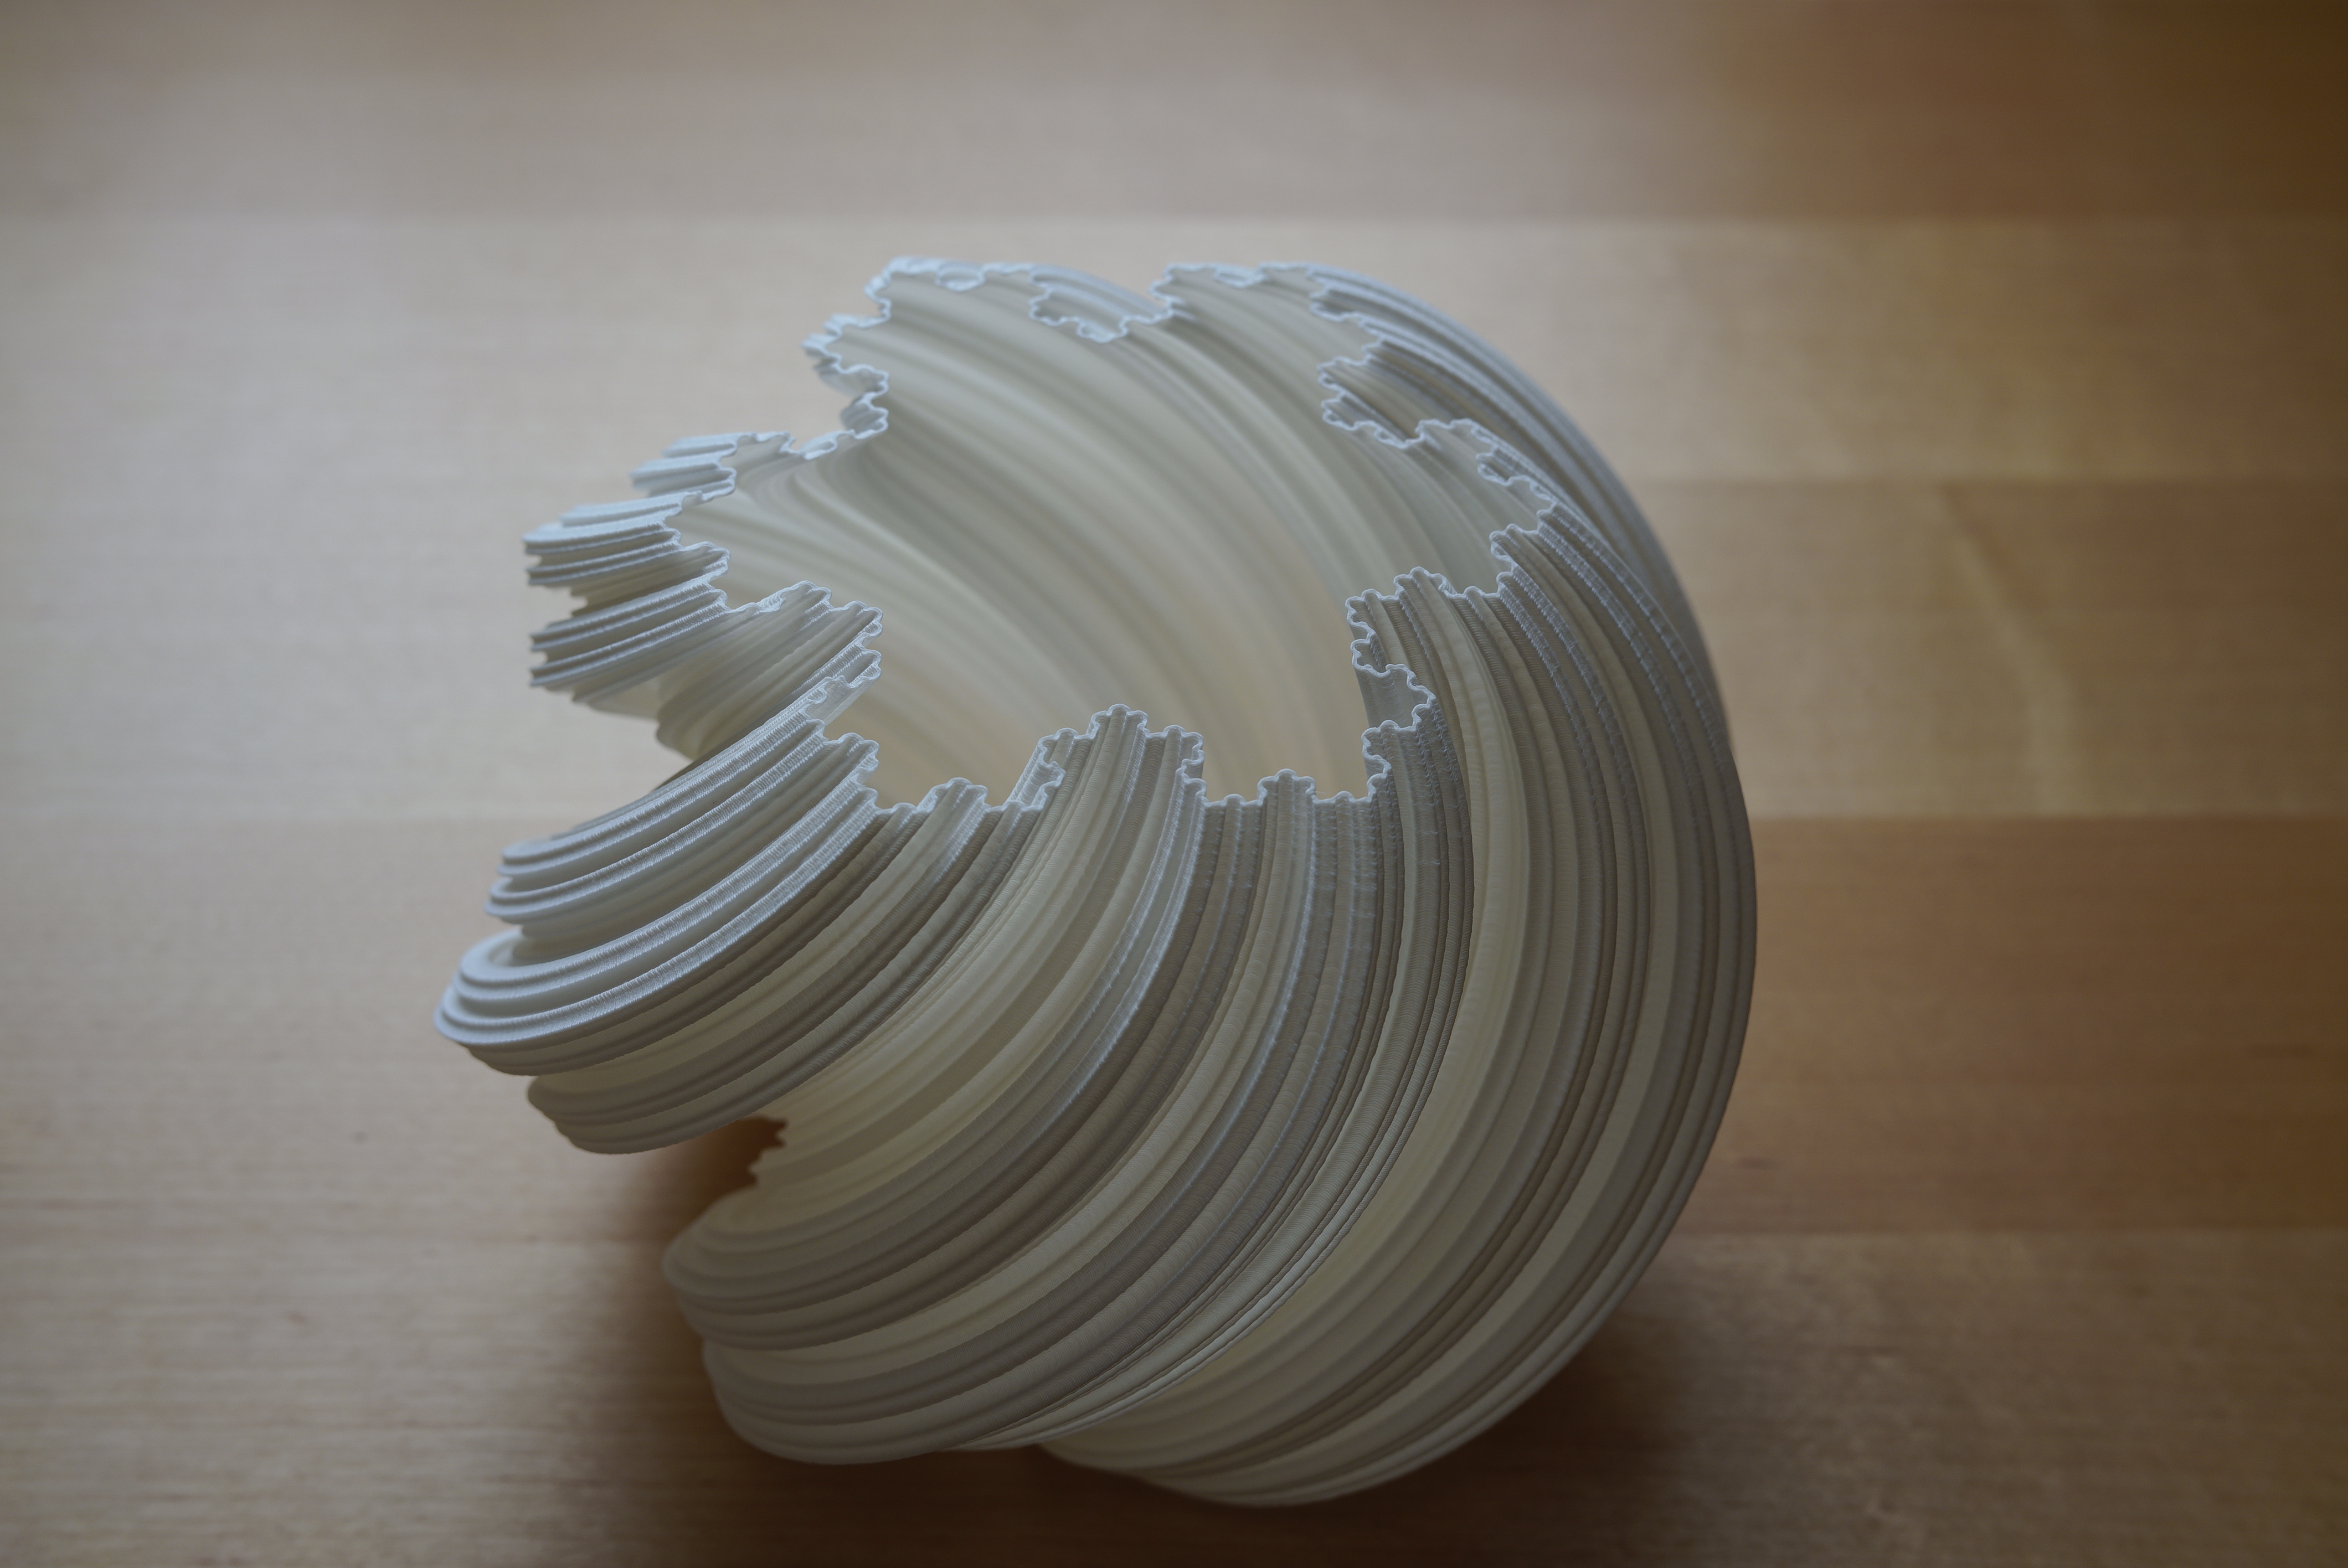
\includegraphics[width=\linewidth]{img/fractal.JPG}
  \caption{koch snowflake pot}
  \label{fig:fractal}
\end{figure}

\subsection{振動による図柄表示}
Pythonの持つ豊富なライブラリを用いれば,あらゆるデータをモデリングのために活用できる.
Figure\ref{fig:audrey}は,OpenCVのライブラリを用いて,モノクロ写真から,ある座標でのピクセルの濃さを抽出,その値を振動の振幅に重みとしてかけている.
白のプレートを印刷後,黒の樹脂で振動パターンを印刷している.その結果,ミクロでは不規則な振動が,マクロでは写真に見える状況を実現している.
従来のCADによる造形では,写真を参考にして造形を行うことはできるが,写真データを直接扱うことはできなかった.
Pythonを用いて造形を行う恩恵により,いままでよりも多彩なデータソースを扱うことができる.
\begin{figure}[htbp]
  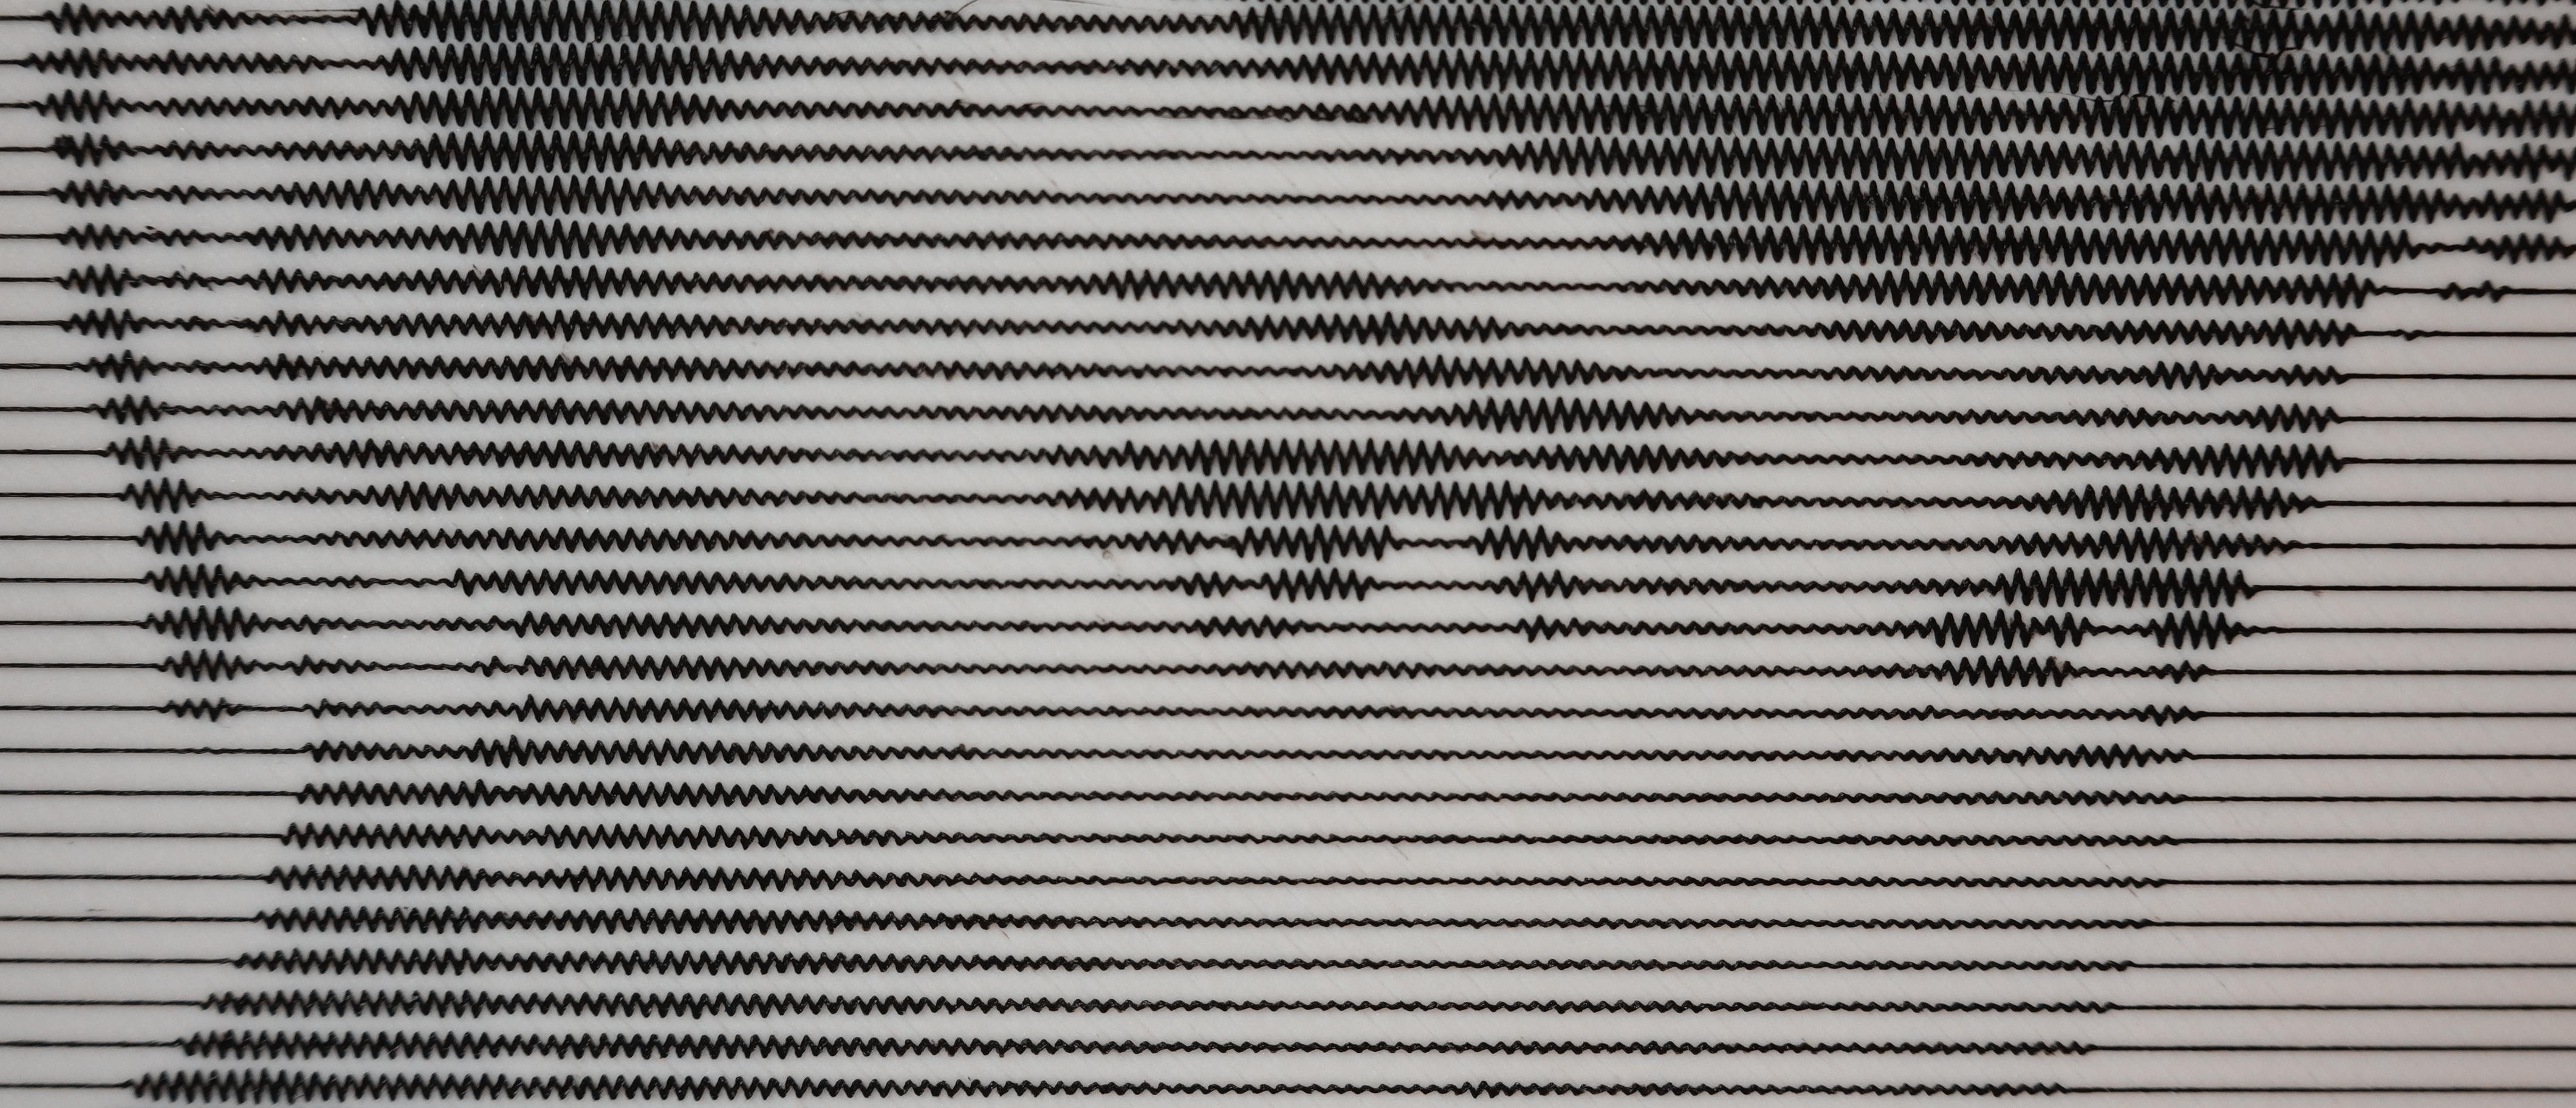
\includegraphics[width=\linewidth]{img/audrey_2.jpg}
  \caption{画像の振動パターン化}
  \label{fig:audrey}
\end{figure}

\subsection{インフィル}
他のG-code Modelingに対して,G-coordinatorが持つ大きな特徴のひとつとして,Fig.\ref{fig:infill}に示すようなインフィルを利用できることが挙げられる.
インフィルを利用できるようになると,実用性を意識したものを作成することができる.
現在は,line infiil, gyroid infillの二種類を利用可能である.

以下のコードをfor文の中に記述することで,最初の20レイヤーにインフィルを付与することができる.
\begin{lstlisting}
if height<20:
    gyroid = gc.gyroid_infill(wall, infill_distance = 2)
    full_object.append(gyroid)
\end{lstlisting}

ここで,wallは外枠を表すPathクラスのオブジェクトである.
gyroid\_infill関数はインフィルを計算する関数であり,外枠のパスを入力として,その内部を埋めるパスを返す関数である.
ただし,インフィルは一本の曲線で表されるものではなく,複数のパスがまとまって,1レイヤー分のインフィルが構成されているため,
厳密には関数からの返り値として返されるのはPathListクラスのオブジェクトである.
しかし,PathListクラスのオブジェクトもPathクラスと同様に印刷設定の指定などができるため,ユーザはPathオブジェクトと同じように扱うことができ,
そのクラスの違いを大きく意識する必要性は少ない.
\begin{figure}[htbp]
  \includegraphics[width=\linewidth]{img/infill_case.JPG}
  \caption{底部にインフィルを付与した小物トレー}
  \label{fig:infill}
\end{figure}

\section{ユーザフィードバックと評価}
ユーザビリティは,新しいソフトウェアの発展において重要な要素となる.
本研究では,G-coordinatorのユーザビリティを評価するために,ユーザにアンケートを実施した.
以下に,G-coordinatorユーザからのフィードバックを示す.
\begin{quote}
  GUIアプリのお陰でプログラム初心者でも使えて大変感謝してます。また、グラスホッパーのように高価なソフトウェアを使用することなくパラメトリックデザインのプリントができるので嬉しいです。
\end{quote}

\begin{quote}
  VBAのfullcontrolから移植して利用しています。サンプル集とビュアーがこれほどありがたいものかと感じています。無償で公開いただいていることに感謝しています。
\end{quote}

\begin{quote}
  すごく面白い。普通のmodeling+slicerと違って、編み物をしていくような感じ。普通のプリントだとヘッドを押し付けて積層するけど、柔らかくなったフィラメントを置いていく感じ。
\end{quote}

\begin{quote}
  面白いけど自由自在に思うような形を作るのは難しい。数学の知識が必要になってしまう。
\end{quote}

自由度の高いG-code Modelingの手法を広く普及させる目的に沿って,G-coordinatorをオープンソース化したことがユーザからの評価につながっている.
しかし,同時に造形の難しさについても指摘されている.これには主に二つの側面がある.一つは造形コードを書く難しさ.
この点については,G-coordinatorでは数多くのサンプルコードを提供している他,公式ドキュメント\cite{gcoordinator}で造形コードを作るためのクイックスタートも示している.
もう一つは,形状を数学的(関数として)表現する難しさがある.この課題に対しては,現時点ではまだ解決策を確立することができていない.

\section{将来展望}
\subsection{開発中のテスト機能}
G-coordinatorを用いて様々な造形を可能にするためにいくつかの機能を開発中である.
何れの機能も既に現在のG-coordinator ver3.0.0にはアルファ版の機能として実装されている,
\subsubsection{数式処理}
\ref{sec:mathmaticalShape}節に示すように,G-coordinatorは数理的な形状を実現させることが非常に得意である.
現在は,さらにその点を生かすべく,様々な関数やクラスを開発中である.
具体的な例として,陽関数のプロットやパスの生成は容易である一方で,陰関数のプロットは高い難易度を伴う.
この課題に対処するため,numpyのmeshgridを活用し,陰関数によって表現された曲線や曲面をより容易に生成できる枠組みを開発中している.
この取り組みにより,より広範で複雑な数学的表現を容易に扱えるようになり,研究や応用上での有用性が向上することが期待される.

\subsubsection{多軸制御}
多軸3Dプリンタの制御においては,座標に加えてノズルの傾きなど,より複雑な要素が造形プロセスに関与するため,その難易度は著しく高まる.
この課題に対処するため,より使いやすく効果的な多軸造形が可能となるようなフレームワークの開発を進めている.

具体的には,クォータニオン(四元数)を活用したノズルの姿勢制御の開発に焦点を当てている.
現行のG-coordinatorの多軸制御手法では,オイラー角や回転行列を使用して姿勢制御を行っている.
それに対し,クォータニオンを導入することで,ジンバルロックなどの特異点を回避しつつ,より柔軟で安定した姿勢制御が可能となる.\cite{yamaguchi1991}
さらに,計算量が削減され,処理時間が短縮されるという利点もある.

新たな手法による多軸制御G-codeの生成においても積極的に取り組んでおり,これによりユーザがより容易に多軸造形を行える環境を提供することを目指している.

\subsubsection{スライス機能}
G-coordinatorは基本的にすべてコードを用いて造形を行う.
しかし,工業的な形状の造形をコードのみで行うことは難しい.
そこで,G-coordinatorにはstlデータをスライスする関数も用意している.

\begin{lstlisting}
  wall = slice(mesh, height*0.2)
\end{lstlisting}
このように,スライス関数にスライス対象のメッシュとスライスする高さを入力することで,スライスした結果のパス(正確にはPathListオブジェクト)が出力される.
純粋なスライスソフトとは異なり,スライスしたパスに対して,個別の印刷設定をマニュアルで付与することができる.
しかし,現在実装しているスライスアルゴリズムではスライスの計算時間が比較的長いことや,トップ/ボトムの表面を手動で設定しなければならない等の問題もあり,まだ完全な実用段階ではない.
将来的には,前節で述べた多軸制御と絡めて,多軸マシンのためのスライス機能もサポートする予定である.

\subsection{ソフトウェアの開発方針}

G-coordinatorは,数学とコードにより,いままで出来なかった形状を実現する一方で,同時に,
ユーザには多少の数学的知識と,プログラムに関するスキルを要求するものであり,参入のための障壁は比較的高いと言わざるをえない.
そこで,現在想定しているG-coordinatorの将来像は大きく分けて二つある.

一つは,Processingなどを代表とするビジュアルアートを実物化させるためのソフトウェアとしての活用である.
Processingとは,プログラムを書いて画面上に図形や形状を描画することができるソフトウェアである.
それに対して,G-coordinatorは,実際に触れるものを作り出せるため,Processingの3次元版となり得る.
これにより,アーティストやデザイナーは数学的なアルゴリズムを用いて,従来不可能だった美しい形状を3Dプリンティングで具現化することが可能になる.

もう一つは,G-coordinatorが数理的な形状に得意な性質を生かし,物理シミュレーションや計算力学を応用して形状を実物化させるソフトウェアとしての利用である.
例えば,トポロジー最適化のアルゴリズムをG-coordiantorの内部で実装し,最適化計算からG-code生成までをシームレスに行うことができるソフトウェアの実現も期待できる.
これにより,エンジニアや科学者は複雑な物理的な現象をシミュレートし,それを具現化するのにG-coordinatorを活用できる.

プログラムを使った3D形状の生成と制御が主眼となる点で,どちらの展望も共通している.

\section{結論}

MEX型3Dプリンタユーザにとって,CAD などの造形手段と,印刷のための調整を行うスライサを同時に置き換える新たな手段としてのG-coordinatorのポテンシャルについて述べた.
スライスソフトに比べて,全部を機械任せにできない欠点はあるものの,裏を返せば,3Dプリンタの挙動の細部までマニュアル操作可能という大きな利点がある.
あらゆる人々に最も自由度の高いG-code Modelingを提供するG-coordiantorは,数学とプログラムの力を駆使して新しい形状を実現するための強力なツールとして,今後の3D プリント分野でさらなる進化が期待される.


\section{謝辞}
田中浩也先生(慶応義塾大学)には多くの助言をいただくとともに,本論文の掲載料を提供していただいた.
また,G-coordinatorの多軸制御の開発において,反保紀昭氏に助言とコード提供をいただいた.
両名の協力がなければ,本研究を今日の形で公表することはできなかった.この場を借りて感謝を申し上げる.

\bibliographystyle{unsrt} % 引用のスタイルを選択
\bibliography{references}     % BibTeXファイルの名前(拡張子なし)

\section{付録}
以下に円柱を造形するためのサンプルコードを示す.ただし,以下のコードはG-coordinator  のver3以降で動作することに注意されたい.

\begin{lstlisting}
  import numpy as np
  import gcoordinator as gc
  
  LAYER = 100
  full_object=[]
  for height in range(LAYER):
      arg = np.linspace(0, 2*np.pi, 100)
      x = 10 * np.cos(arg)
      y = 10 * np.sin(arg)
      z = np.full_like(arg, (height+1) * 0.2)
      wall = gc.Path(x, y, z)
      full_object.append(wall)
  gc.gui_export(full_object)
\end{lstlisting}


\end{twocolumn}
\end{document}
